\mode*
\section{Pointers and Arrays}

\begin{frame}
  \begin{minipage}[t]{.44\linewidth}
    \includegraphics[width=\textwidth]{array2-c}
  \end{minipage}
  \begin{minipage}[t]{.52\linewidth}
    \includegraphics[width=\textwidth]{array2-2-c}\tikzmark{array2-2}
    \mode<beamer>{
      \begin{tikzpicture}[remember picture,overlay]
        \node at ($(pic cs:array2-2)+(-.68,.91)$) [ellipse,opacity=.4,red,draw,thick,minimum
        width=1cm] {};
      \end{tikzpicture}}
    \mode<article>{
      \begin{tikzpicture}[remember picture,overlay]
        \node at ($(pic cs:array2-2)+(-.9,1.4)$) [ellipse,opacity=.4,red,draw,thick,minimum
        width=1.5cm] {};
      \end{tikzpicture}
      C automatically scales pointer arithmetic so that it works correctly, by
      incrementing/decrementing by the correct number of bytes. For example, at line 11,
      the value of \texttt{pa} is \texttt{1008}, and the value of \texttt{a} is
      \texttt{1000}. But the result of ``\texttt{pa - a}'' is \texttt{2} rather than
      \texttt{8}. This means \texttt{pa} is \emph{two ints} ahead of \texttt{a}.}
  \end{minipage}
  \begin{center}
    \mode<beamer>{ 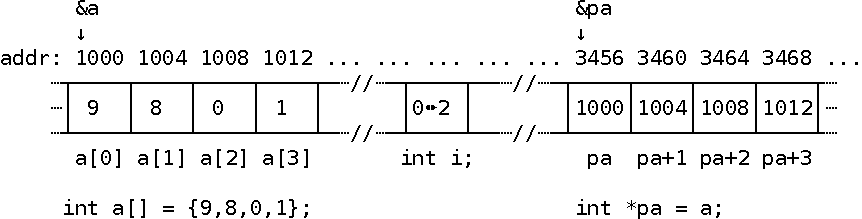
\includegraphics[width=\textwidth]{array2-3} }%
    \mode<article>{ 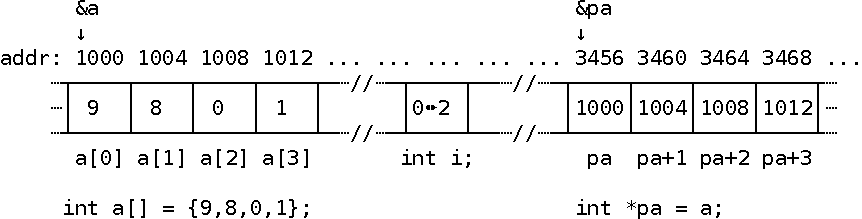
\includegraphics[width=.6\textwidth]{array2-3} }
  \end{center}
\end{frame}

\begin{frame}{Passing Arrays to Functions}
  \begin{block}{}
    When passing an array to a function, C will automatically change the array into a
    pointer.
  \end{block}  
  \begin{minipage}{.55\linewidth}
    \begin{center}
      \mode<beamer>{ \includegraphics[width=\textwidth]{array3-1-c} }%
      \mode<article>{ \includegraphics[width=.6\textwidth]{array3-1-c} }
    \end{center}
  \end{minipage}\hfill
  \begin{minipage}{.4\linewidth}
    \begin{center}
      \mode<beamer>{ 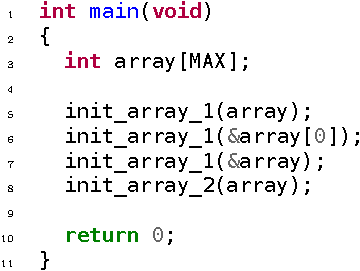
\includegraphics[width=\textwidth]{array3-2-c} }%
      \mode<article>{ 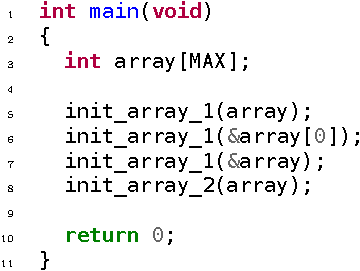
\includegraphics[width=.6\textwidth]{array3-2-c} }
    \end{center}
  \end{minipage}
\end{frame}

\begin{frame}[fragile]{Arrays of Pointers}
  \begin{center}
    \mode<beamer>{ \includegraphics[width=.7\textwidth]{array4-c} }%
    \mode<article>{ \includegraphics[width=.5\textwidth]{array4-c} }
  \end{center}
\end{frame}

\paragraph*{Once you've declared an array, you can't reassign it. Why?}
[\url{https://stackoverflow.com/questions/17077505/string-pointer-and-array-of-chars-in-c}]

Consider an assignment like

\begin{ccode}
char *my_str = "foo"; // Declare and initialize a char pointer.
my_str = "bar"; // Change its value.
\end{ccode}

The first line declares a char pointer and ``aims'' it at the first letter in \texttt{foo}. Since \texttt{foo} is a string constant, it resides somewhere in memory with all the other constants. When you reassign the pointer, you're assigning a new value to it: the address of \texttt{bar}. But the original string, \texttt{foo}, remains unchanged. You've moved the pointer, but haven't altered the data.

\emph{When you declare an array, however, you aren't declaring a pointer at all. You're reserving a certain amount of memory and giving it a name}. So the line

\begin{ccode}
char c[5] = "data";
\end{ccode}

starts with the string constant \texttt{data}, then allocates 5 new bytes, calls them \texttt{c}, and copies the string into them. You can access the elements of the array exactly as if you'd declared a pointer to them; arrays and pointers are (for most purposes) interchangeable in that way.

\emph{But since arrays are not pointers, you cannot reassign them}. You can't make
\texttt{c} ``point'' anywhere else, because it's not a pointer; it's the name of an area of
memory. For example,

\begin{ccode}
char c[5] = "data";
char b[5] = "beta";
b = c; /* Wrong! 'b[]' cannot be reassigned (pointing to elsewhere). */
\end{ccode}

\begin{frame}[fragile=singleslide]{How not to Use Pointers}
  \begin{iblock}{Life is complicated enough, don't make it worse}
\begin{ccode}
/* Point to the first element of the array. */
data_ptr = &array[0];

/* Get element #0, data_ptr points to element #1. */
value = *data_ptr++;

/* Get element #2, data_ptr points to element #2. */
value = *++data_ptr;

/* Increment element #2, return its value.
   Leave data_ptr alone. */
value = ++*data_ptr;
\end{ccode}
  \end{iblock}
  \begin{tikzpicture}[remember picture,overlay]
    \node at ($(current page.center)+(4.5,-2)$) [opacity=.2,red,scale=10] {\bad};
  \end{tikzpicture}  
\end{frame}

\begin{frame}[fragile]
  \begin{iblock}{Just don't do it}
\begin{ccode}
void copy_string(char *p, char *q)
{
  while (*p++ = *q++);
}
\end{ccode}
  \begin{tikzpicture}[remember picture,overlay]
    \node at ($(current page.center)+(2,-2)$) [opacity=.2,red,scale=10] {\bad};
  \end{tikzpicture}  
  \end{iblock}
\end{frame}

% https://ocw.mit.edu/courses/electrical-engineering-and-computer-science/6-s096-effective-programming-in-c-and-c-january-iap-2014/lecture-notes/

% https://ocw.mit.edu/courses/electrical-engineering-and-computer-science/6-088-introduction-to-c-memory-management-and-c-object-oriented-programming-january-iap-2010/lecture-notes/

\mode<all>
%%% Local Variables:
%%% mode: latex
%%% TeX-master: "c-b"
%%% End:
